%сделать восклицательный знак
\documentclass[a4paper,12pt,fleqn]{article} % добавить leqno в [] для нумерации слева

%%% Работа с русским языком
\usepackage{cmap}					% поиск в PDF
\usepackage{mathtext} 				% русские буквы в формулах
\usepackage[T2A]{fontenc}			% кодировка
\usepackage[utf8]{inputenc}			% кодировка исходного текста
\usepackage[english,russian]{babel}	% локализация и переносы

%%% Дополнительная работа с математикой
\usepackage{amsmath,amsfonts,amssymb,amsthm,mathtools} % AMS
\usepackage{icomma} % "Умная" запятая

%% Номера формул
%\mathtoolsset{showonlyrefs=true} % Показывать номера только у тех формул, на которые есть \eqref{} в тексте.
%\usepackage{leqno} %Нумерация формул слева

%% Шрифты
\usepackage{euscript}	 % Шрифт Евклид
\usepackage{mathrsfs} % Красивый матшрифт


%% Свои команды
\DeclareMathOperator{\sgn}{\mathop{sgn}}

%% Перенос знаков в формулах (по Львовскому)
\newcommand*{\hm}[1]{#1\nobreak\discretionary{}
{\hbox{$\mathsurround=0pt #1$}}{}}

%%% Заголовок
\author{}
\title{}
\date{}



%%% Теоремы
%\theoremstyle{definition}
%\newtheorem{case}{Задача}[section]
%\renewcommand{\thecase}{\arabic{case}}

%\theoremstyle{definition} % "Определение"
%\newtheorem{corollary}{Пункт}[case]
%\newtheorem{problem}{Задача}[section]
%\renewcommand{\thecorollary}{\asbuk{corollary}}

\usepackage{multicol} % Несколько колонок


%%% Работа с картинками
\usepackage{graphicx}  % Для вставки рисунков
\graphicspath{{images/}{images2/}}  % папки с картинками
\setlength\fboxsep{3pt} % Отступ рамки \fbox{} от рисунка
\setlength\fboxrule{1pt} % Толщина линий рамки \fbox{}
\usepackage{wrapfig} % Обтекание рисунков текстом

%%% Работа с таблицами
\usepackage{array,tabularx,tabulary,booktabs} % Дополнительная работа с таблицами
\usepackage{longtable}  % Длинные таблицы
\usepackage{multirow} % Слияние строк в таблице

%%% Страница
%\usepackage{extsizes} % Возможность сделать 14-й шрифт
\usepackage{geometry} % Простой способ задавать поля
\geometry{top=20mm}
\geometry{bottom=20mm}
\geometry{left=30mm}
\geometry{right=20mm}
%
\usepackage{fancyhdr} % Колонтитулы
\pagestyle{fancy}
\renewcommand{\headrulewidth}{0.1mm}  % Толщина линейки, отчеркивающей верхний колонтитул
%\lfoot{Нижний левый}
%\rfoot{Нижний правый}
\rhead{Глава \thesection}
%\chead{Верхний в центре}
%\lhead{}
% \cfoot{Нижний в центре} % По умолчанию здесь номер страницы

\usepackage{setspace} % Интерлиньяж
%\onehalfspacing % Интерлиньяж 1.5
%\doublespacing % Интерлиньяж 2
%\singlespacing % Интерлиньяж 1

\usepackage{soulutf8} % Модификаторы начертания
\usepackage{bm} % Модификатор начертания для математики

%\usepackage{tikz} % Работа с графикой
%\usepackage{pgfplots}
%\usepackage{pgfplotstable}
%\usepackage[utf8]{inputenc}
%\usetikzlibrary{arrows}


\usepackage{hyperref}
\usepackage[usenames,dvipsnames,svgnames,table,rgb]{xcolor}
\hypersetup{				% Гиперссылки
	unicode=true,           % русские буквы в раздела PDF
	pdftitle={Заголовок},   % Заголовок
	pdfauthor={Автор},      % Автор
	pdfsubject={Тема},      % Тема
	pdfcreator={Создатель}, % Создатель
	pdfproducer={Производитель}, % Производитель
	pdfkeywords={keyword1} {key2} {key3}, % Ключевые слова
	colorlinks=true,       	% false: ссылки в рамках; true: цветные ссылки
	linkcolor=blue!55!red,          % внутренние ссылки
	citecolor=green,        % на библиографию
	filecolor=magenta,      % на файлы
	urlcolor=blue          % на URL
} 
\usepackage{datetime}
\newdateformat{onlyyear}{\THEYEAR}
\newdateformat{defaultdate}{\THEDAY~\monthname[\THEMONTH] \THEYEAR~г.}

\usepackage{multicol} % Несколько колонок

\usepackage{indentfirst} % Красная строка

\usepackage{tikz} % Работа с графикой
\usepackage{pgfplots} %взять данные из соседнего файла и построить по ним что-либо
\usepackage{pgfplotstable}
\usetikzlibrary{fadings}
\usetikzlibrary{decorations}
\usepgflibrary{decorations.pathmorphing}

\tikzfading[name=fade out, inner color=transparent!0,
outer color=transparent!100]

\usepackage[utf8]{inputenc}
\usetikzlibrary{arrows}
\usepackage{tcolorbox}
\usepackage{lipsum}
\tcbuselibrary{breakable}

%\usetikzlibrary{calc}

\usepackage{xparse}
\NewDocumentCommand{\definition}{mm}{ \textbf{Определение.} \textit{#1} --- #2 \vspace{0.3cm}}

\renewcommand{\familydefault}{\sfdefault}
\usepackage{float}

\usepackage{relsize}
\newcommand{\bigem}[1][1]{\text{\larger[#1]{\color{blue!55!red}{ \textbf{$ ! $}}}}}


\begin{document} % конец преамбулы, начало документа
	
\tableofcontents

\newpage


\section{Угрозы в области физической безопасности}

\begin{tcolorbox}[colback=blue!40!red!10!,colframe=blue!40!red]


В результате изучения главы студент должен \textbf{знать} основные угрозы в области обеспечения физической безопасности предприятия в сферах защиты жизни и здоровья физических лиц, обеспечения сохранности финансовых и иных материальных ценностей, а также объектов недвижимости; \textbf{уметь} сопоставлять основные угрозы с типовыми мерами обеспечения физической защиты бизнеса; \textbf{владеть} методами обеспечения физической безопасности предприятия с применением различных типов защиты, а также расчетом экономических показателей себестоимости различных вариантов охраны.

\end{tcolorbox}


\subsection{Угроза жизни и здоровью физических лиц}

Важным \textit{условием успешного функционирования любого предприятия на рынке} является защита от возникающих угроз, среди которых особую опасность представляют незаконные действия физических лиц. Последствия их действий непредсказуемы: от хищения имущества до создания чрезвычайных ситуаций на объекте. В этих условиях безопасность любого субъекта рынка осуществляется на основе принципов «разумной достаточности», «эффективность – стоимость», а также разработанной в теории и применяемой на практике концепции физической безопасности предприятия.

В рамках единой политики безопасности организации физическая безопасность является основным структурным элементом, направленным на сохранение собственности, жизни и здоровья персонала, финансовых ресурсов.\\

\definition{Физическая безопасность организации} {совокупность правовых норм, организационных мер и инженерно-технических решений, направленных на защиту важных интересов и ресурсов предприятия (объекта) от угроз злоумышленных противоправных действий физических лиц (нарушителей или злоумышленников).}

Как правило, она включает в себя силы подразделений безопасности и охраны объекта, комплекс инженерно-технических средств охраны, а также режим, установленный на объекте. Система физической защиты не должна препятствовать нормальному функционированию организации, ее технологическим процессам.

Угрозы в области физической безопасности существенно различаются по своей тяжести и зависят от возможностей и способностей нарушителя. В качестве \textit{основных видов угроз в области физической безопасности} принято различать  (см. рисунок \ref{image1}): 

\begin{itemize}
\item Чрезвычайные ситуации (пожар, разрушение, затопление, авария, хищение опасных веществ, массовые инфекционные заболевания и отравления людей и т.п.);
\item Промышленный шпионаж;
\item Угрозы физическому лицу (сотрудникам): причинение вреда здоровью, причинение увечий, создание угроз для жизни;
\item Хищение или порча имущества;
\item Несанкционированный съем информации, содержащей государственную, служебную или коммерческую тайны;
\item Снижение эффективности функционирования и устойчивости развития предприятия.
\end{itemize}

\begin{figure}
\centering
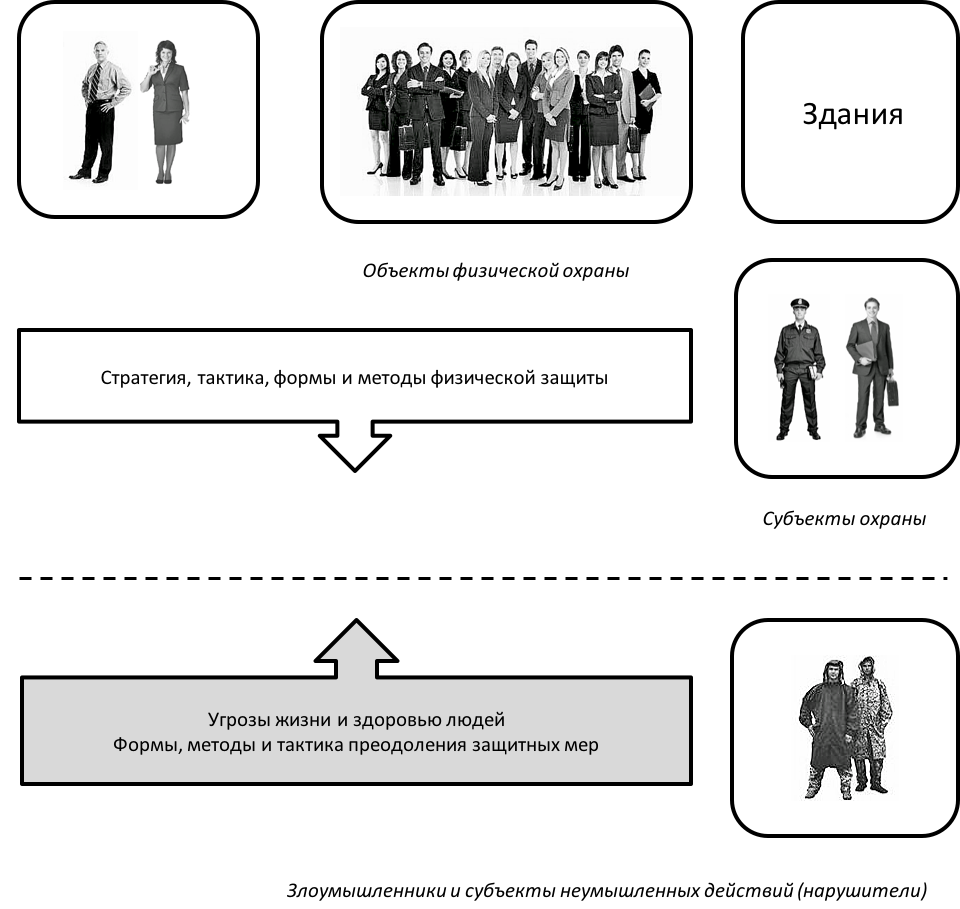
\includegraphics[scale=0.7]{img1}
\caption{Угроза и защита в области обсепечения физической безопасности}
\label{image1}
\end{figure}

К \textit{объектам физической охраны} относятся:
\begin{itemize}
\item Собственники бизнеса и члены их семей;
\item Топ-менеджеры и персонал предприятия, места их нахождения;
\item Товарно-материальные и финансовые ценности;
\item Служебная документация, составляющая коммерческую и иную тайну, а также объекты интеллектуальной собственности;
\item Объекты недвижимости, а также объекты обеспечения жизнедеятельности предприятия (энергообеспечение, теплоснабжение, водоснабжение и др.).
\end{itemize}

Как правило, объектами физического насилия стано­вятся руководители предприятий или сотрудники, зани­мающие определенное должностное положение (принимают управленческие и кадровые решения, имеют право подписи финансовых документов, участвуют в пла­нировании работы предприятия, заключении сделок, ин­вестиционных проектах и пр.). Вместе с тем, отдельные сотрудники могут становиться объектами физических посягательств и в силу различных конфликтных ситуаций.\\

\begin{tcolorbox}[colback=blue!55!red!5!,colframe=blue!55!red,enforce breakable,% use only breakable in the real world!
	pad at break=1mm, title=Кейс 1. Действия обиженного сотрудника]
	
7 ноября 2012 г. юрист Дмитрий Андреевич Виноградов, 1983 года рождения приехал на работу в компанию «Ригла» (г. Москва) с рюкзаком, в котором находилось специальное снаряжение и боеприпасы, и двумя ружейными чехлами, в которых находились карабины «Сайга» и «Benelli».

В головном офисе фармацевтической компании он беспрепятственно прошел пост охраны, включая металлодетектор. Зашел в мужской туалет на 3-м этаже, где переоделся в военизированный костюм, расчехлил и подготовил к стрельбе оружие. По дороге с третьего на четвертый этаж Виноградов встретил случайно проходившего сотрудника компании и расстрелял его. Затем он прошел к кабинету № 400 и эффектно вошел туда с двумя карабинами наперевес, где начал расстреливать всех присутствовавших. На месте им было убито 4 человека (двое мужчин и две женщины). Двое тяжело раненных лиц были доставлены в клинику, где один из потерпевших скончался от полученных ранений в грудную клетку. Силами службы безопасности «Риглы» Виноградов был задержан и обезоружен. По предварительным данным следствия, он совершил преступление на почве неразделенной любви, а жертвами стали коллеги любимой девушки, которые иронично относились к чувствам Виноградова. К убийству нескольких человек преступник готовился практически год. В это время он не только купил длинноствольное оружие и посещал стрелковый клуб, но и обращался к психиатру с жалобой на проблемы с психикой. 

Начальник охраны «Риглы» был уволен, но это не помогло вернуть к жизни погибших.

\begin{itemize}
\item[{\color{blue!55!red}\Huge {  $ ? $}} \quad]   Сообщите свое мнение о том, как можно было предотвратить преступление.
\end{itemize}	
	
\end{tcolorbox}

\renewcommand{\theenumi}{\arabic{enumi}}
\renewcommand{\labelenumi}{(\theenumi)}

В общем плане к угрозам физической безопасности личности относятся: 
\begin{itemize}
	\item Похищения и угрозы похищения сотрудников, членов их семей и близких родственников; 
	\item Убийства, сопровождаемые насилием, издевательствами и пытками; 
	\item Психологический террор, угрозы, запугивание, шантаж, вымогательство; 
	\item Нападение с целью завладения денежными средствами, ценностями и документами. 
\end{itemize}


\begin{tcolorbox}[colback=blue!40!red!1!,colframe=blue!40!red,enforce breakable,% use only breakable in the real world!
	pad at break=1mm, title=Вопросы и задания для самоконтроля]
	\begin{itemize}
		\item[{\color{blue!55!red}\Huge { $ ? $}} ]  Дайте определение понятия «потеря деловой репутации предприятия» в рамках его защиты от угроз в области финансовой безопасности.
		\item[{\color{blue!55!red}\Huge {  $ ? $}} ] Расскажите об угрозах, которые могут нанести ущерб предприятию вследствие нарушения правил ведения бухгалтерской отчетности.
		\item[{\color{blue!55!red}\Huge {  $ ? $}} ] Сообщите об угрозах нарушения правил валютно-экспортных операций.
		\item[{\color{blue!55!red}\Huge {  $ ? $}} ] Расскажите об операциях, подлежащих обязательному контролю, при осуществлении контроля в целях ПОД/ФТ.
		\item[{\color{blue!55!red}\Huge {  $ ? $}} ] Расскажите об угрозе нарушения порядка и правил осуществления контроля в целях ПОД/ФТ субъектом данного вида деятельности.
		
	\end{itemize}		
\end{tcolorbox}







\end{document}